% This file was created by matlab2tikz.
%
\definecolor{mycolor1}{rgb}{0.12941,0.12941,0.12941}%
%
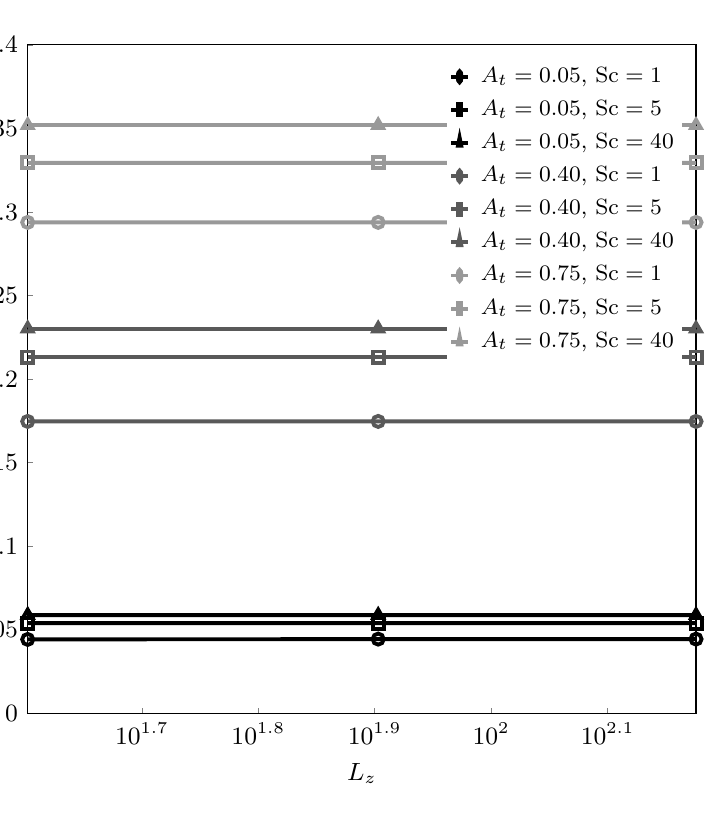
\begin{tikzpicture}[trim axis left,trim axis right]

\begin{axis}[%
width=11.252in,
height=7.131in,
at={(1.887in,0.962in)},
scale only axis,
clip=true,
xmode=log,
xmin=40,
xmax=150,
xminorticks=true,
xlabel style={font=\color{mycolor1}},
xlabel={$L_z$},
ymin=0,
ymax=0.4,
ylabel style={font=\color{mycolor1}},
ylabel={$\omega_r^{\max}$},
axis background/.style={fill=white},
legend style={legend cell align=left, align=left},
clip=true,
clip mode=individual,
axis lines=box,
xtick pos=bottom,
ytick pos=left,
tick align=inside,
major tick length=2pt,
width=0.7\linewidth,
height=0.7\linewidth,
every axis/.append style={font=\fontsize{9}{9}\selectfont},xlabel style={font=\fontsize{9}{9}\selectfont},title style={font=\fontsize{9}{9}\selectfont},
legend style={font=\fontsize{8}{9}\selectfont,inner sep=1pt,row sep=1pt,column sep=2pt,nodes={scale=1.00},draw=none},legend image post style={xscale=0.35},
legend columns=1,
scaled x ticks=false,
tick label style={/pgf/number format/fixed,/pgf/number format/precision=2},
every x tick label/.append style={font=\fontsize{9}{9}\selectfont\color{black}},
every y tick label/.append style={font=\fontsize{9}{9}\selectfont\color{black}},
,,
colormap={sigmamap}{rgb(0.0000)=(0.0200,0.1880,0.3800); rgb(0.1000)=(0.0743,0.3456,0.5616); rgb(0.2000)=(0.1918,0.4980,0.7060); rgb(0.3000)=(0.3890,0.6708,0.8226); rgb(0.4000)=(0.7552,0.8682,0.9228); rgb(0.5000)=(0.9690,0.9689,0.9689); rgb(0.6000)=(0.9425,0.8044,0.7614); rgb(0.7000)=(0.8767,0.4910,0.4020); rgb(0.8000)=(0.7869,0.2866,0.2470); rgb(0.9000)=(0.6186,0.1239,0.1568); rgb(1.0000)=(0.4040,0.0000,0.1220)}
]
\addplot [color=black, line width=1.4pt, mark=o, mark options={solid, black}]
  table[row sep=crcr]{%
40	0.0441818899132971\\
80	0.0443785920268873\\
150	0.0443788288459807\\
};
\addlegendentry{$A_t=0.05,\,\mathrm{Sc}=1$}

\addplot [color=black, line width=1.4pt, mark=square, mark options={solid, black}]
  table[row sep=crcr]{%
40	0.0539144465284922\\
80	0.0539217634643817\\
150	0.0539217643577263\\
};
\addlegendentry{$A_t=0.05,\,\mathrm{Sc}=5$}

\addplot [color=black, line width=1.4pt, mark=triangle, mark options={solid, black}]
  table[row sep=crcr]{%
40	0.0587557038467365\\
80	0.0587569222384135\\
150	0.0587569222433593\\
};
\addlegendentry{$A_t=0.05,\,\mathrm{Sc}=40$}

\addplot [color=white!35!black, line width=1.4pt, mark=o, mark options={solid, white!35!black}]
  table[row sep=crcr]{%
40	0.17465935459338\\
80	0.174659108645165\\
150	0.174659112011224\\
};
\addlegendentry{$A_t=0.40,\,\mathrm{Sc}=1$}

\addplot [color=white!35!black, line width=1.4pt, mark=square, mark options={solid, white!35!black}]
  table[row sep=crcr]{%
40	0.213159885846062\\
80	0.213159891007819\\
150	0.21315989116325\\
};
\addlegendentry{$A_t=0.40,\,\mathrm{Sc}=5$}

\addplot [color=white!35!black, line width=1.4pt, mark=triangle, mark options={solid, white!35!black}]
  table[row sep=crcr]{%
40	0.230189224406083\\
80	0.230189219537165\\
150	0.230189220202142\\
};
\addlegendentry{$A_t=0.40,\,\mathrm{Sc}=40$}

\addplot [color=white!60!black, line width=1.4pt, mark=o, mark options={solid, white!60!black}]
  table[row sep=crcr]{%
40	0.293783329990469\\
80	0.293783998411243\\
150	0.293783951621569\\
};
\addlegendentry{$A_t=0.75,\,\mathrm{Sc}=1$}

\addplot [color=white!60!black, line width=1.4pt, mark=square, mark options={solid, white!60!black}]
  table[row sep=crcr]{%
40	0.329384688278383\\
80	0.329384673579652\\
150	0.329384676395385\\
};
\addlegendentry{$A_t=0.75,\,\mathrm{Sc}=5$}

\addplot [color=white!60!black, line width=1.4pt, mark=triangle, mark options={solid, white!60!black}]
  table[row sep=crcr]{%
40	0.351902158061809\\
80	0.351902147902805\\
150	0.351902148322234\\
};
\addlegendentry{$A_t=0.75,\,\mathrm{Sc}=40$}

\node[overlay,right, align=left, inner sep=0, font=\color{mycolor1}]
at (rel axis cs:-0.25,1.15) {$(a)$};
\end{axis}
\end{tikzpicture}%